%!TEX root = main.tex

\section{Introduction}
In this work, we study the noise sensitivity of the state-of-the-art for route flow estimation for mobility cyber-physical systems (CPS). Route flow estimation on road networks is a critical problem for mobility CPS, as any real-time prediction and control applications require accurate and reliable estimates of the state of the road network. Previous work has demonstrated the promise of using area-based sensors such as cellular towers as inputs to a convex optimization formulation of the problem, along with a projected first-order method that scales well to large city-scale networks \cite{Wu2015}. Importantly, the work's introduction of the concept of \textit{cellpath} (sequences of cell tower regions) helps to cope with the underdetermined-ness of the problem. However, the numerical results are based off of noiseless synthetic data, which makes the strong but common assumption that vehicles are connected to the closest cell tower throughout their trajectory (i.e. voronoi tessellations of cell tower regions) \cite{Voronoi1908}. The real world is seldom so kind.

We extend upon the previous work by analyzing the sensitivity of the estimation procedure to structured noise. In particular, we consider noise from a generative model based off of a handoff model for cellular base stations, which includes hysteresis margins for handoffs, load balancing, and random interference.
 
\subsection{Route flow estimation problem}
The route flow estimation problem (illustrated in Figure \ref{fig:example-setup}) is as follows: for a road network $G=(V,E)$, let $\mathcal{R}$ denote the set of $n$ routes that vehicles take. We denote $f$ to be the cellpath flow (measured), $d$ to be the origin-destination (OD) flow (measured), $b$ the link flow (measured), and $x \in \mathbb{R}^n$ the route flow (unknown). We are given the linear operators relating the sensor measurements ($f,d,b$) to the route flow $x$ ($U,T,A$, respectively), that is $Ax=b, Tx=d, Ux=f$. We wish to recover $x$ from the flow measurements of the sensors.

With the exception of the noise model, we follow the same assumptions as in \cite{Wu2015}: static setting, and continuous and well-posed cellpaths.

\begin{figure}[h!]
  \centering
    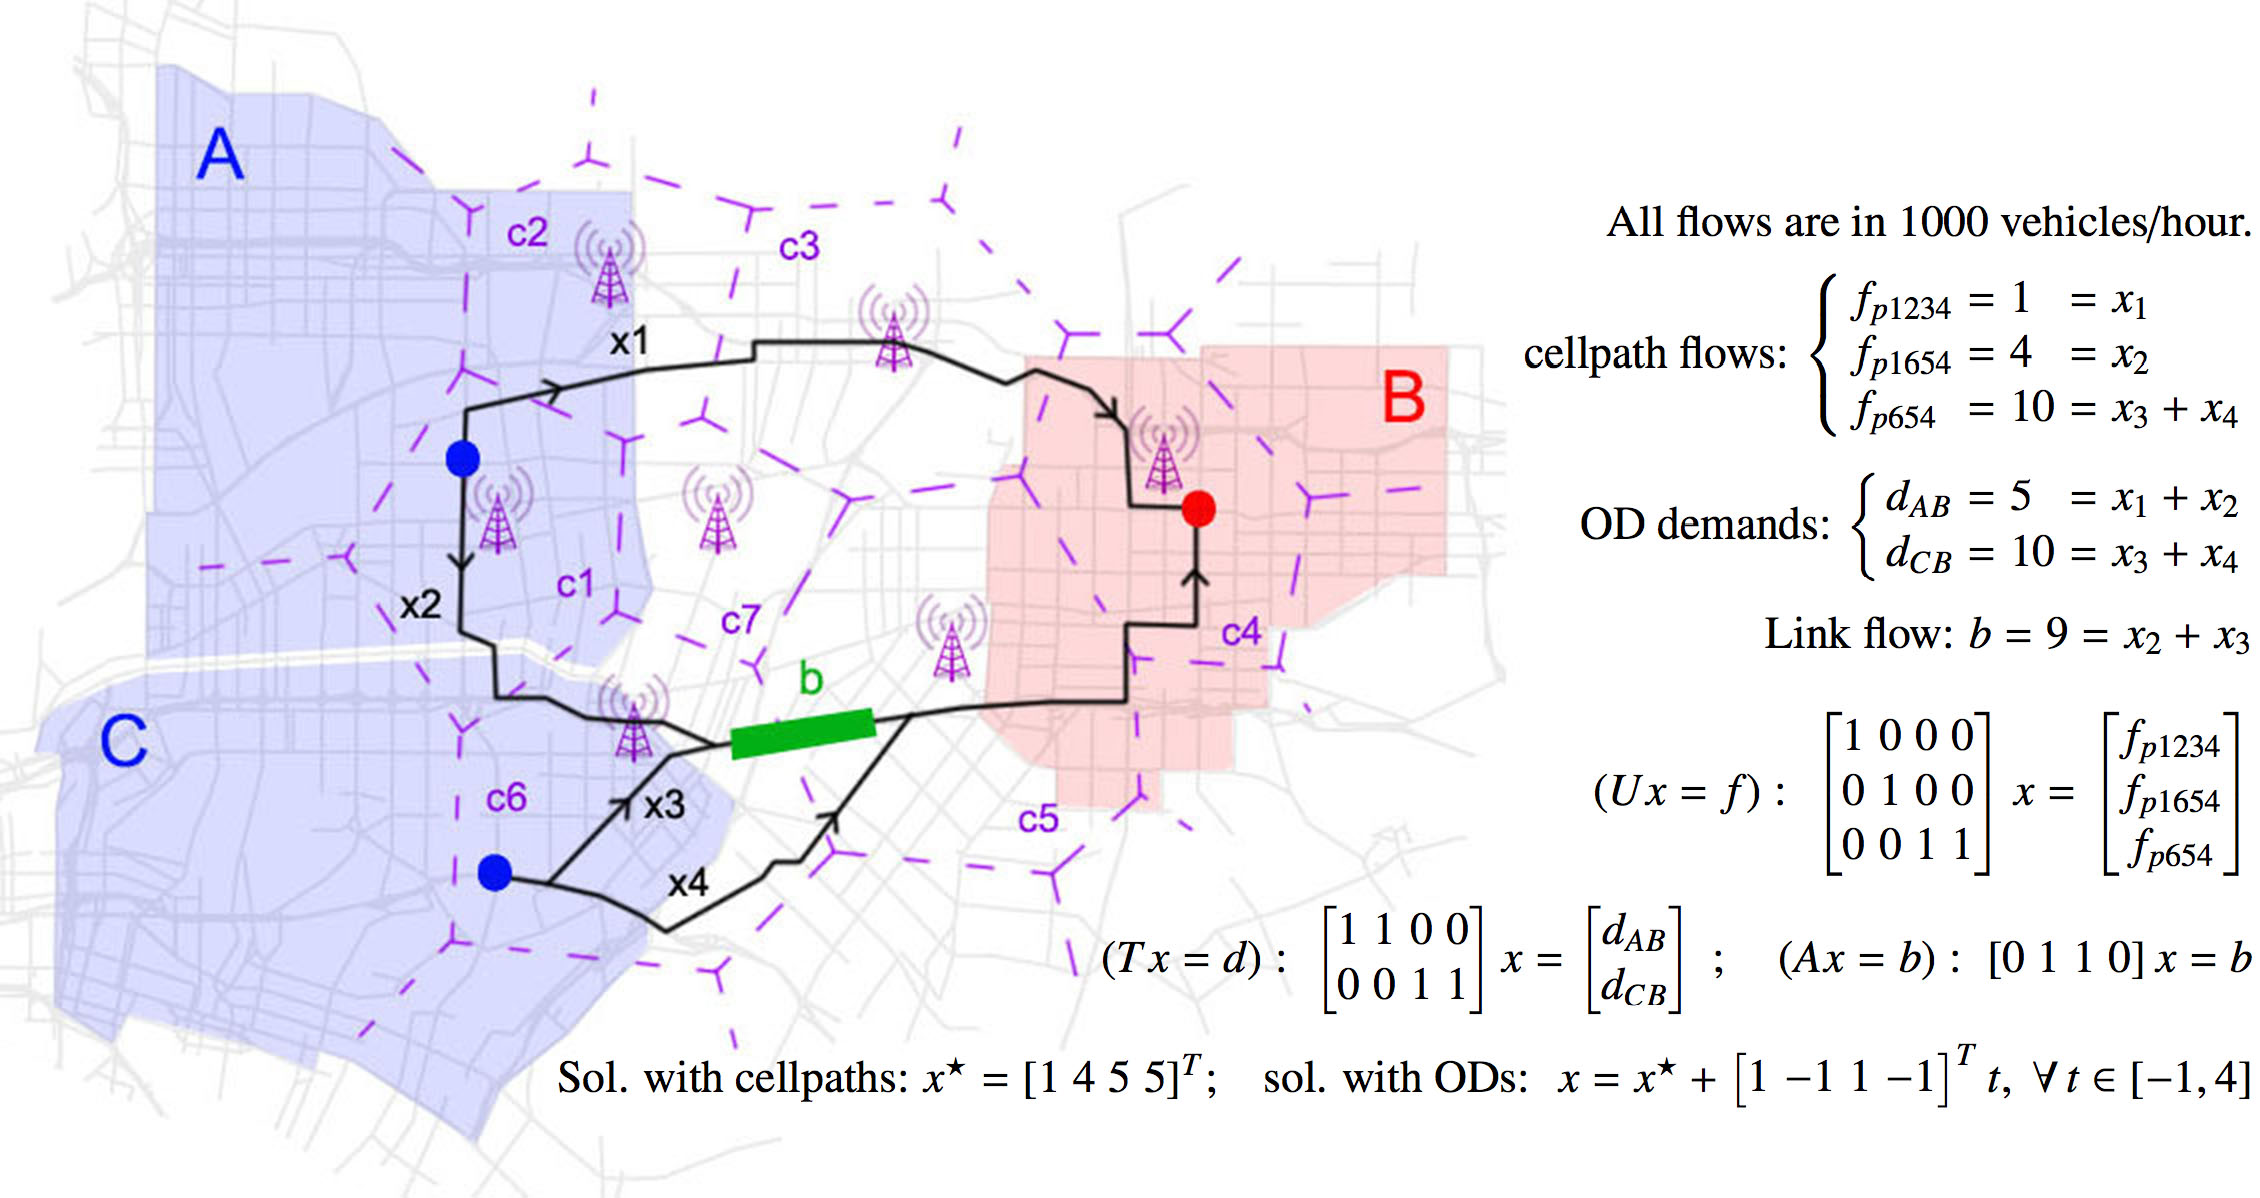
\includegraphics[width=0.47	\textwidth]{figures/setup}
  \caption{\footnotesize{In this illustration, we have two origins A and C ({\color{blue}blue}) and one destination B ({\color{red}red}). We have routes $r_1,r_2,r_3,r_4$ with flows $x=(x_1,x_2,x_3, x_4)$ such that $r_1,r_2$ go from A to B and $r_3,r_4$ go from C to B. Cells $c_1,\cdots,c_7$ are shown in {\color{magenta} purple} dashed regions. Since route $r_1$ goes through cells $c_1,c_2,c_3,c_4$, its associated cellpath is $p_{1234}$. Similarly, routes $r_2,r_3,r_4$ have cellpaths $p_{1654},p_{654},p_{654}$ respectively. Let $f_{p1234},\,f_{p1654},\,f_{p654}$ be the cellpath flows (obtained from cellular network data), \emph{i.e.} there are $f_{p1234}$=1000~veh/h going through $c_1,c_2,c_3,c_4$. Let $d_{AB}$ and $d_{CB}$ be the OD demands and $b$ be the link flow ({\color{green}green}, from loop detectors). Without considering data from cellpaths, the problem has \emph{one degree of freedom} and is \emph{underdetermined} with only the OD demands as data.}}
  \label{fig:example-setup}
\end{figure}

\subsection{Related works}


